\pdfoutput=1
\pdfcompresslevel=9
\pdfinfo
{
    /Author (Aleksy Barcz)
    /Title (Implementation aspects of graph neural networks)
    /Keywords (Graph neural networks, classification, graph processing, recursive neural networks)
}
%\documentclass[a4paper,polish,onecolumn,oneside,floatssmall,11pt,titleauthor,wide,openright]{mwrep}
%\usepackage[scale={0.7,0.8},paper=a4paper,twoside]{geometry}
\documentclass[a4paper,onecolumn,oneside,12pt,wide,floatssmall]{mwrep} % 11pt w szablonie, 12pt dla TimesNewRoman
\usepackage{amsmath}
\usepackage{amsfonts}
\usepackage{amssymb}
\usepackage{amsthm}
\usepackage{bookman}
\usepackage{bm}		% bold math symbols

\usepackage{geometry}
\usepackage[utf8x]{inputenc}
\usepackage[T1]{fontenc}
% \usepackage{t1enc}
% \usepackage[pdftex, bookmarks]{hyperref}
%\usepackage[pdftex, bookmarks=false]{hyperref}
\usepackage[pdftex, bookmarks=true, colorlinks=true,linkcolor=black,urlcolor=blue,citecolor=black]{hyperref}
%\def\url#1{{ \tt #1}}
\usepackage{url} % linki url w bibliografii
\usepackage{alltt}
\usepackage{booktabs} % eleganckie tabelki
\usepackage{mathtools} % wyrównane macierze, wymaga texlive-latex3
\usepackage{bm} % pogrubione greckie litery

\usepackage{listings}

\usepackage{pslatex} %Times New Roman

% marginesy
\textwidth\paperwidth
\advance\textwidth -55mm
\oddsidemargin-0.9in
\advance\oddsidemargin 33mm
\evensidemargin-0.9in
\advance\evensidemargin 33mm
\topmargin -1in
\advance\topmargin 13mm
\setlength\textheight{48\baselineskip}
\addtolength\textheight{\topskip}
\marginparwidth15mm

\clubpenalty=10000 % to kara za sierotki
\widowpenalty=10000 % nie pozostawia wdów
\brokenpenalty=10000 % nie dzieli wyrazów pomiędzy stronami
\sloppy

\tolerance4500
\pretolerance250
\hfuzz=1.5pt
\hbadness1450

\linespread{1.3}	% interlinia 1.5 linii

% dotfill with smaller dots
\makeatletter
\newcommand \Dotfill {\leavevmode \cleaders \hb@xt@ .25em{\hss .\hss }\hfill \kern \z@}
\makeatother

% ŻYWA PAGINA
\renewcommand{\chaptermark}[1]{\markboth{\scshape\small\bfseries \
#1}{\small\bfseries \ #1}}
\renewcommand{\sectionmark}[1]{\markboth{\scshape\small\bfseries\thesection.\
#1}{\small\bfseries\thesection.\ #1}}
\newcommand{\headrulewidth}{0.5pt}
\newcommand{\footrulewidth}{0.pt}
\pagestyle{uheadings}

\usepackage[pdftex]{color,graphicx}
\usepackage[english]{babel}
\usepackage[usenames,dvipsnames]{xcolor} % kolory dla listingow kodu

% \textheight232mm
% \setlength{\textwidth}{\textwidth}
% \setlength{\oddsidemargin}{\evensidemargin}
% \setlength{\evensidemargin}{0.3cm}
\usepackage[sort, compress]{cite}

%\usepackage{multibib}
%\newcites{bk,st,doc,web}{Książki i~artykuły,Standardy i~zalecenia,Dokumentacja produktów,Publikacje i~serwisy internetowe}

\theoremstyle{definition}
\newtheorem{defn}{Definition}[section]
\newtheorem{exmp}{Example}[section]

\theoremstyle{plain}% default
\newtheorem{thm}{Theorem}[section]
\newtheorem{lem}[thm]{Lemma}
\newtheorem{prop}[thm]{Hipothesis}
\newtheorem*{cor}{Conclusion}

\theoremstyle{remark}
\newtheorem*{rem}{Remark}
\newtheorem*{note}{Remark}
\newtheorem{case}{Case}

\definecolor{ListingBackground}{rgb}{1,1,1}

\begin{document}

% kody źródłowe wplatane w tekst
\lstdefinestyle{incode}
{
basicstyle={\footnotesize},
keywordstyle={\bf\footnotesize\color{black}},
commentstyle={\em\footnotesize\color{gray}},
numbers=left,
stepnumber=5,
firstnumber=1,
numberfirstline=true,
numberblanklines=true,
numberstyle={\sf\tiny},
numbersep=10pt,
tabsize=2,
xleftmargin=17pt,
framexleftmargin=3pt,
framexbottommargin=2pt,
framextopmargin=2pt,
framexrightmargin=0pt,
showstringspaces=true,
backgroundcolor={\color{ListingBackground}},
extendedchars=true,
% title=\lstname,
captionpos=b,
% abovecaptionskip=1pt,
% belowcaptionskip=1pt,
frame=tb,
framerule=0pt,
}

% kody źródłowe z podpisem
\lstdefinestyle{outcode}
{
basicstyle={\footnotesize},
keywordstyle={\bf\footnotesize\color{black}},
commentstyle={\em\footnotesize\color{gray}},
numbers=left,
stepnumber=5,
firstnumber=1,
numberfirstline=true,
numberblanklines=true,
numberstyle={\sf\tiny},
numbersep=10pt,
tabsize=2,
xleftmargin=17pt,
framexleftmargin=3pt,
framexbottommargin=2pt,
framextopmargin=2pt,
framexrightmargin=0pt,
showstringspaces=true,
backgroundcolor={\color{ListingBackground}},
extendedchars=true,
% title=\lstname,
captionpos=b,
% abovecaptionskip=1pt,
% belowcaptionskip=1pt,
frame=tb,
framerule=0.1pt,
}

\pagenumbering{roman}
\renewcommand{\baselinestretch}{1.0}
\raggedbottom
%
\begin{titlepage}
    % Strona tytułowa
    \vbox to\textheight{\hyphenpenalty=10000
    \begin{center}
	\begin{tabular}{p{107mm} p{9cm}}
	    \begin{minipage}{9cm}
	      \begin{center}
	      Politechnika Warszawska \\
	      Wydział Elektroniki i~Technik Informacyjnych \\
	      Instytut Informatyki
	      \end{center}
	    \end{minipage}
	    &
	    \begin{minipage}{8cm}
	    \begin{flushleft}
	      Rok akademicki 2012/2013
	    \vspace*{2.75\baselineskip}
	    \end{flushleft}
	    \end{minipage} \\
	\end{tabular}
	\vspace*{2.5\baselineskip}
	\begin{center}
		\includegraphics[height=3.5cm,width=3.5cm]{img/PW_logo.png}
	\end{center}
	\vspace*{2.2\baselineskip}{\Large \MakeUppercase{Praca dyplomowa magisterska}\par}
	\vspace{2\baselineskip}{\large Aleksy Stanisław Barcz\par}
	\vspace*{2\baselineskip}{\LARGE Implementation aspects of graph neural networks\par}

	\vspace*{7\baselineskip}
	\hfill\mbox{}\par\vspace*{\baselineskip}\noindent
	\begin{tabular}[b]{@{}p{3cm}@{\ }l@{}}
	    {\large\hfill } & {\large }
	\end{tabular}
	\hfill
	\begin{tabular}[b]{c}
		Opiekun pracy: \\
		{mgr inż. Zbigniew Szymański}
	\end{tabular}\par
	\vspace*{5\baselineskip}
    \begin{tabular}{p{\textwidth}}
    \begin{flushleft}
	\begin{minipage}{7cm}
	Ocena: \Dotfill
	\par\vspace{2.5\baselineskip}
	\Dotfill
	\vspace{0.5\baselineskip}
	\par\noindent
	\centerline{Podpis Przewodniczącego}
	\centerline{Komisji Egzaminu Dyplomowego}\par
	\end{minipage}
    \end{flushleft}
    \end{tabular}
    \end{center}}

    % Życiorys
    \newpage\thispagestyle{empty}
    \begin{tabular}{p{4cm} p{20cm}}
    \begin{minipage}{4cm}
    \includegraphics[height=4.8cm,width=4cm]{img/myphoto_cropped.png}
    \end{minipage}
    &
    \begin{minipage}{20cm}
    \begin{flushleft}
    \par\noindent\vspace{1\baselineskip}
    \begin{tabular}[h]{l l}
    {\normalsize Kierunek:} & Informatyka\\
    {\normalsize Specjalność:} & Inżynieria systemów informatycznych
    \end{tabular}
    \par\noindent\vspace{2\baselineskip}
    \begin{tabular}[h]{l r}
    {\normalsize Data urodzenia:} & {\normalsize 1988.01.28} \\
    {\normalsize Data rozpoczęcia studiów:} & {\normalsize 2012.02.20}
    \end{tabular}
    \par\noindent\vspace{2\baselineskip}
    \end{flushleft}
    \end{minipage}
    \end{tabular}
    \vspace*{1\baselineskip}
    \begin{center}
	{Życiorys}\par\bigskip
    \end{center}

    \noindent
	Ukończyłem XXVIII LO im. J.Kochanowskiego w Warszawie, w klasie o profilu matematyczno - informatycznym. Studia inżynierskie ukończyłem w lutym 2012 roku na kierunku Informatyka na Wydziale Elektroniki i Technik Informacyjnych Politechniki Warszawskiej. W trakcie studiów I i II stopnia brałem udział w wymianach studenckich programu Athens na Katholieke Universiteit Leuven \emph{(Fundamentals of artificial intelligence)} oraz w Télécom ParisTech \emph{(Emergence in complex systems)}.
    \par
    \vspace{2\baselineskip}
    \hfill\parbox{15em}{{\small\Dotfill}\\[-.3ex]
    \centerline{Podpis studenta}}\par
    \vspace{3\baselineskip}
 	{\noindent\MakeUppercase{Egzamin dyplomowy}} \par\bigskip\bigskip
    \par\noindent\vspace{1.5\baselineskip}
    Złożył egzamin dyplomowy w dniu \Dotfill 2013~r.
    \par\noindent\vspace{1.5\baselineskip}
    z wynikiem \Dotfill
    \par\noindent\vspace{1.5\baselineskip}
    Ogólny wynik studiów: \Dotfill
    \par\noindent\vspace{1.5\baselineskip}
    Dodatkowe wnioski i uwagi Komisji: \Dotfill
    \par\noindent\vspace{1.5\baselineskip}
    \Dotfill
    \par\noindent\vspace{1.5\baselineskip}
    \Dotfill

    % Streszczenie
    \newpage\thispagestyle{empty}
    \vspace*{2\baselineskip}
    \begin{center}
	{\large \MakeUppercase{Summary}}\par\bigskip
    \end{center}

    {\noindent
	This thesis describes the process of implementation of a Graph Neural Network, a classifier capable of classifying data represented as graphs. Parameters affecting the classifier efficiency and the learning process were identified and described. Implementation details affecting the classifier efficiency were described. Important similarities to other connectionist models used for graph processing were highlighted.
	}
    \vspace*{1\baselineskip}

    \noindent{Keywords}: {Graph neural networks, classification, graph processing, recursive neural networks}
    \par
    \vspace{4\baselineskip}

	\begin{center}
	\line(1,0){250}
	\end{center}

    \begin{center}
	{\large \MakeUppercase{ASPEKTY IMPLEMENTACYJNE GRAFOWYCH SIECI NEURONOWYCH}}\par\bigskip
    \end{center}
    {\noindent
	Praca stanowi raport z samodzielnej implementacji klasyfikatora typu Graph Neural Network (grafowa sieć neuronowa), pozwalającego na klasyfikację danych o strukturze grafowej. W ramach pracy zidentyfikowane zostały istotne dla klasyfikatora parametry, wpływające na przebieg procesu uczenia się klasyfikatora oraz na jakość uzyskanych wyników. Opisane zostały szczegóły implementacyjne klasyfikatora istotne dla jego działania. Klasyfikator został przedstawiony w kontekście podobnych rozwiązań w celu ukazania ścisłych powiązań między istniejącymi modelami przetwarzania danych o strukturze grafowej, opartymi na sieciach neuronowych.
	}
	
    \vspace*{1\baselineskip}

    \noindent{Słowa kluczowe}: {Grafowe sieci neuronowe, klasyfikacja, przetwarzanie grafów, rekursywne sieci neuronowe}

\end{titlepage}

% ex: set tabstop=4 shiftwidth=4 softtabstop=4 noexpandtab fileformat=unix filetype=tex spelllang=pl,en spell:


\tableofcontents
% \addcontentsline{toc}{chapter}{{Przedmowa1}{vii}}{vii}

% \chapter*{Spis tablic, rysunków i~wydruków}
% \listoftables
% \listoffigures
% \lstlistoflistings

%\setlength{\baselineskip}{7mm}
\newpage
\pagenumbering{arabic}
\setcounter{page}{1}


\chapter{Introduction}
The Graph Neural Network model is a connectionist classifier capable of classifying graphs. Most of the other existing neural network-based graph classifiers, such as RAAM~\cite{pollack1990recursive} or  LRAAM~\cite{sperduti1994labelling} and all solutions basing on them are capable of processing certain types of graphs only, in most cases DAGs (directed acyclic graphs) or DPAGs (directed positional acyclic graphs).
Several solutions were invented to deal with cyclic graphs, such as introducing a delay in the LRAAM encoding tree~\cite{goulon2005hopfield} or techniques mapping cyclic directed graphs to "recursive equivalent" trees~\cite{bianchini2003backpropagation}.
The problem of nonpositional graphs was also addressed by several authors, either by creating domain-specific encodings used to enforce a defined order on graph nodes~\cite{ivanciuc2003canonical} or by introducing various modifications to the classifier~\cite{bianchini2005recursive}.
However, most of the solutions dealing with cyclic and nonpositional graphs either complicate the classifier model, enlarge the input dataset or (in case of cycles) may result in information loss. The Graph Neural Network model can directly process most types of graphs, including cyclic, acyclic, directed, undirected, positional and nonpositional, which makes it a flexible solution.
There is a conceptual similarity between the GNN model and Graph Machines~\cite{goulon2005learning}, however the GNN model adapt a different learning and backpropagation schema which simplifies processing different types of graphs.
This thesis describes the steps of implementation of a GNN classifier, including some details which were not described in the original article~\cite{scarselli2009graph}. The classifier was implemented in GNU Octave with two ideas in mind: providing a simple interface (similar to that of the Neural Networks toolbox) and maximum flexibility, that is the possibility of processing each kind of data that the theoretical model could deal with. The process of training a GNN and classification results were presented in detail.



\chapter{Domains of application\label{chap:domains}}
This chapter presents domains where data is organized into a structured form, that is form of sequences or graphs. The necessity of processing differently such kinds of data arose from the structure of the data itself. To present this difference we must first summarize what is the task of classification and regression in the most common meaning in the data processing domain. A common statistical classifier (which later on is called a \emph{vectorial} classifier) takes as input \emph{samples} from a given \emph{dataset}, representing real world objects, and associates each sample with a \emph{category}. The samples are fixed-length vectors of numeric values. Each position in such a vector represents a \emph{feature} of the sample, which is quantified by a real or integer value. The mapping from features to positions in the vector is fixed and must hold for each sample in the dataset. The category is represented by a non-empty fixed-length vector of integer values, where once again the position of each value is meaningful (we can say it's a \emph{positional} representation). For the regression task, a vector of real (or integer) values is associated with each sample instead of a category. The domain of vectorial classifiers is well developed and includes, among other solutions, neural networks, support vector machines, naïve Bayes classifiers and random forests.

In the case of graph processing, the nature of the data is different. Each \emph{sample} is represented by a \emph{graph}. A \emph{dataset} may consist of a single or several graphs. Each graph consists of nodes, connected with edges. Each node can be described by its \emph{label}, a fixed-length vector of reals. Each edge can also be labelled, with a fixed-length vector of reals of different size. Edges can be directed or undirected.

\begin{figure}
\begin{center}
	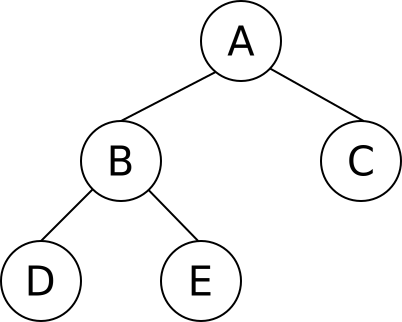
\includegraphics[scale=0.4]{img/tree}
	\caption{A simple binary tree}
	\label{fig:simple_tree}
\end{center}
\end{figure}

An example of a simple graph was presented in Fig.~\ref{fig:simple_tree}. If such a graph was to be used as input for a vectorial classifier, it would be necessary to transform the structured representation into a plain vector. It could be accomplished in several ways, one of the most obvious would be to perform a preorder walk on the tree and list the node labels in the order they were visited. Such a walk would result in the representation $[A,B,D,E,C]$. It can be seen that the explicit information about node adjacency was lost. Instead, the information is provided implicitly, according to a coding which must be known a priori to properly interpret such a vectorial representation. That means that a model learning to classify such graph representations would have to \emph{learn} the encoded relationship, instead of benefiting from it from the beginning to learn other, unknown and interesting relationships affecting the samples category. The resulting learning task becomes even harder if such sequential representations contain \emph{long-distance relationships}. Different encodings from structured data to vectors exist, however, they all share that flaw.

Moreover, the inadequacy of simple vector representation becomes even more apparent when the graph structure becomes more complicated. First of all, if edge labels are present in the vector representation, the representation becomes a mix of data belonging to two different entities - nodes and edges. Once again the classifier doesn't know which part of the data corresponds to the first entity and which to the other. The same applies to directed and undirected edges. If two edges in a graph are connected by a directed edge, presumably one of the nodes in the relation has got a larger impact on the other than vice versa. On the contrary, an undirected or bidirectional edge edge implies an equal impact of both nodes on each other. What if a graph contains both types of edges? How should one type of edges be distinguished from the other one? Secondly, let's consider the case of cyclic dependencies. Even if a meaningful representation of the graph is built ignoring cycles, e.g. by constructing a minimum spanning tree, some explicit information about connections is lost. An example of such data are chemical compounds containing groups of atoms forming cyclic bonds. Another problem lies in the positional nature of vectorial data. If a representation is built by simply storing node labels one after another, such a representation becomes vulnerable to any reordering of the children of a node. An additional effort must be made to assure a \emph{consistent ordering} of the potentially difficult to order data, while the ordering of the children of a node may be irrelevant in the dataset considered.

It can be seen that in order to properly process structured data, a different approach must be used. The data should be processed in a way that exploits properly the information contained in its structure - by means of building a sufficient representation or by processing the structured data directly. 

Graph-oriented models based on neural networks were successfully applied in various domains, including chemistry, pattern recognition and natural language processing. In the domain of computer-aided drug design the most important problem to solve is to predict the properties of a molecule prior to synthesizing it. All molecules with a negative prediction can be discarded automatically, reducing the costs of the subsequent laboratory experiments which can focus on the molecules with a positive prediction only~\cite{goulon2005hopfield}. This is the case of QSAR (quantitative structure-activity relations) and QSPR (quantitative structure-property relations). While traditional processing methods consist of extraction and selection of features from the molecules descriptions, the molecules can be easily represented as undirected graphs and processed with a graph-oriented model~\cite{goulon2007predicting}~\cite{goulon2005learning}.

The next domain of interest is document mining. As the amount of XML-formatted information increases rapidly, the problem of determining if a document can be assigned to a given category becomes crucial. As an XML document can be viewed as semi-structured data, graph-processing models can be successfully applied to this task~\cite{yong2006xml}. Another problem focused on document processing is the web page ranking, where documents and the links between them can be described as structured data. A general ranking model can be implemented as a graph-processing model, which allows exploiting page contents and link analysis simultaneously.~\cite{scarselli2005graph}~\cite{scarselli2009graph}.

In the domain of image processing two pattern recognition tasks can be distinguished. The first is the classification of images, either for industrial applications, control and monitoring, or for querying an image database. The second is object localisation, which may be used e.g. for face localisation. For both tasks an image can be represented as a RAG (Region Adjacency Graph), where image segments are represented as nodes and their adjacency is represented as edges which may contain information about e.g. the distances between adjacent segments. For both tasks graph-processing methods can be used, yielding promising results~\cite{monfardini2006graph}~\cite{bianchini2005recursive}~\cite{quek2011structural}.

Another classic example where structure of the data plays a crucial role in its understanding is the natural language processing. In the unconstrained case, the input data may consists of arbitrarily complex sentences. As a sentence can be transformed into a graph reflecting its syntax, a graph-processing model can be trained to parse such sentences. One of the first graph-processing models was already evaluated on such a task~\cite{pollack1990recursive} and more recent solutions are also present in the literature~\cite{costa2003towards}. 


\chapter{Graph processing models}
\noindent A model considered as fully capable of processing structured data, should be able to:
\begin{enumerate}
	\item build data representation
	\begin{enumerate}
		\item minimal
		\item exploiting sufficiently the structure of the data
		\item adequate for subsequent processing (classification, regression)
	\end{enumerate}
	\item perform classification / regression on the structured data
	\begin{enumerate}
		\item taking into consideration the structure encoded in the representation
		\item with a high generalization capacity
	\end{enumerate}
\end{enumerate}
These two main tasks are often intertwined with each other, as a classification procedure may affect the procedure of representation building and vice versa. It is also possible for a model to focus only on representation building, while leaving the task of processing to a common statistical classifier, such as a support vector machine. Two main families of models capable of processing structured data are the \emph{symbolic} and the \emph{connectionist} family. The first one originates in the artificial intelligence domain and focus on inferring relationships by means of inductive logic programming. The \emph{connectionist} models focus on modelling relationships with the use of interconnected networks of simple units. The different models originating from these two families are:
\begin{enumerate}
	\item inductive logic programming
	\item evolutionary algorithms
	\item probabilistic models: Bayes networks and Markov random fields
	\item graph kernels
	\item neural network models
\end{enumerate}
The main area of interest of this thesis are the connectionist models based on neural networks. The connectionist models make the fewest assumptions about the domain of the dataset and thus provide a potentially most general method for processing structured data.


\chapter{History}
This chapter summarizes the history of connectionist models used for graph processing. All these models originate from the common feed-forward neural networks (FNNs). The history of neural networks begins in 1943 with the McCulloch–Pitts (MCP) neuron model, following with the Rosenblatt perceptron classifier in 1957. During the following three decades, the feed-forward neural network model was developed and until 1988 a conclusive state was reached in all major fields of related research. The FNN model reached maturity in its field of application: classification and regression performed on unstructured positional samples of fixed size. In the '80s a new branch of the neural networks family began to develop - the recurrent neural networks (RNN). The RNN model is capable of processing sequences of varying length (potentially infinite), which makes them suitable for dealing with time-varying sequences or biological samples of various length~\cite{saha2006prediction}. However, one more approach had to be tried before the RNN model was adapted to processing graph data.

\section{Hopfield networks}
One of the earliest attempts to classify structured data with neural networks was using the Hopfield networks~\cite{goulon2005hopfield}. A common application of a Hopfield is an auto-associative memory, which learns to reproduce patterns provided as its input lines (the learned task is $x_i \Rightarrow x_i$, where $x_i$ is a pattern of fixed size $\forall_{i \in [1..N]} |x_i| = n$). Afterwards, when a new sample is presented to the trained network, the network associates it with the most similar pattern it had learned. However, it was discovered, that by using the Hopfield network to reproduce a predefined successor of a pattern instead of the pattern itself, the network can be used as an hetero-associative memory, capable of reproducing sequences of patterns ($x_i \Rightarrow x_{i+1}$). The next step towards graph processing was to use Hopfield networks to learn the task of reproducing \emph{all} the successors (or predecessors) of a node, that is learn the task $x_i \Rightarrow succ[x_i]$, where $succ[x_i]$ are the successors of node $x_i$ and $\forall_i |succ[x_i]| \leq m \cdot |x_i|$, where $m$ is the maximum outdegree of a node in the analyzed graphs. $NIL$ patterns are used as extra successors whenever a considered node $x_i$ has an outdegree smaller than $m$. The last and somehow different application of Hopfield networks was to use a Hopfield network once again as an auto-associative memory, used for retrieving whole graphs. In such case the graph adjacency matrices ($N \times N$) are encoded into a network having $N(N - 1)/2$ neurons~\cite{goulon2005hopfield}. To obtain an adequate generalisation graphs isomorphic to the training set are generated and fed to the network~\cite{kree1988recognition}.

\section{RAAM}
The Recursive Auto-Associative Memory (RAAM) was introduced by Pollack in 1990~\cite{pollack1990recursive}. The RAAM model is a generalisation of the Hopfield network model~\cite{goulon2005hopfield}, providing means to meaningfully encode directed positional acyclic graphs (DPAGs). This type of graphs contains in particular undirected trees, however in the case of directed graphs their structure may be more complex, as long as there are no cycles. A distinctive feature of the RAAM model is that is can be used to encode graphs with labeled terminal nodes (leaves in the case of trees) only. That is, no node other than the terminal nodes of a graph may be labelled. No edge labels are permitted. The most straightforward domain of application for the RAAM model is thus natural language processing, where sentences can be decomposed to syntax graphs.\\
\noindent The RAAM model is capable of:
\begin{itemize}
	\item building compressed representation of structured data
	\item building meaningful representation: similar samples are represented in a similar way
	\item constrained generalisation: representing data absent in the training set
\end{itemize}
The RAAM model is composed of two units: \emph{compressor} and \emph{reconstructor}. Together they form a three-layer feed-forward neural network which works as an auto-associative memory. The \emph{compressor} is a fully connected two-layer neural network with $n$ input lines and $m$ output neurons. The number of output neurons, $m$ determines the size of a single encoded node representation. The number of input lines, $n$ must be a multiple of $m$, such that $n = k \cdot m$, where $k$ is the maximum outdegree of a node in the considered graphs. For each terminal node its representation consists of its original label. For each non-terminal node $i$ its representation, $x_i$ is built by feeding the compressor with encoded representation of the $i$th nodes children. To assure that the compressed representation is accurate and lossless, it is fed to the \emph{reconstructor}. The reconstructor is also a fully connected two-layer neural network, however it has $m$ input lines and $n$ output neurons. It is fed with compressed representations of nodes and produces the original data that was fed to the compressor. This procedure is repeated for all non-terminal nodes of a graph, until all encoded representations can be accurately decoded into original data. More precisely, the representation $x_i$ of the $i$th node of the graph is given by Eq.~\ref{eq:raam_representation}, where $f$ denotes the function implemented by the compressor unit, $l_i$ - the label of $i$th node, $x_{ch_j}$ - the $j$th child node of the $i$th node, $k$ - the maximum outdegree of a node in the graph. An example of a graph that can be encoded using the RAAM model is presented in Fig.~\ref{fig:tree_for_raam}.

\begin{equation}
x_i = \left\{
\begin{array}{l l}
	l_i & \quad \text{if $i$ is terminal} \\
	f(x_{ch_1}, .., x_{ch_k}) & \quad \text{otherwise}
\end{array}
\right.
\label{eq:raam_representation}
\end{equation}

\begin{figure}
\begin{center}
	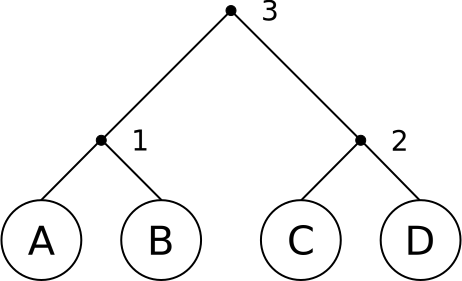
\includegraphics[scale=0.4]{img/tree_for_raam}
	\caption{A sample graph that can be processed using RAAM, only leaves are labelled}
	\label{fig:tree_for_raam}
\end{center}
\end{figure}

To encode the sample graph, first the representations of nodes $1$ and $2$ must be built. The representation of node $1$ is built by feeding the pair of labels $(A, B)$ to the compressor which encodes them into the representation $x_1$. The representation $x_1$ is then fed to the reconstructor, which produces a pair of labels $(A', B')$. If the resulting labels $A'$ and $B'$ are not similar enough to the original labels $A$ and $B$, the error is backpropagated through the compressor-reconstructor three-layer network. Similarly, the pair $(C, D)$ is compressed by the same compressor-reconstructor pair into the representation $x_2$. Then, the pair $(x_1, x_2)$ is once again fed to the compressor, which produces $x_3$, the representation of the root node. This is also the compressed representation of the whole graph, from which the whole graph can be reconstructed by using the reconstructor unit. The training set, consisting of three label pairs, is presented in Fig.~\ref{fig:raam1-3}. The light grey areas denote the compressor network, while the dark grey areas denote the reconstructor. Such a training set (or a larger one if the dataset consists of more than one graph) must be repeatedly processed by the RAAM model in the training phase. When the model is trained, the compression of the whole graph occurs as presented in Fig.~\ref{fig:raam_compression}. Reconstruction of the graph is presented in Fig.~\ref{fig:raam_reconstruction}.

\begin{figure}
\begin{center}
	
\includegraphics[scale=0.4]{img/raam1-3}
	\caption{Training set for the example graph}
	\label{fig:raam1-3}
\end{center}
\end{figure}

\begin{figure}
\begin{center}
	
\includegraphics[scale=0.4]{img/raam_encode}
	\caption{Graph compression using trained RAAM model}
	\label{fig:raam_compression}
\end{center}
\end{figure}

\begin{figure}
\begin{center}
	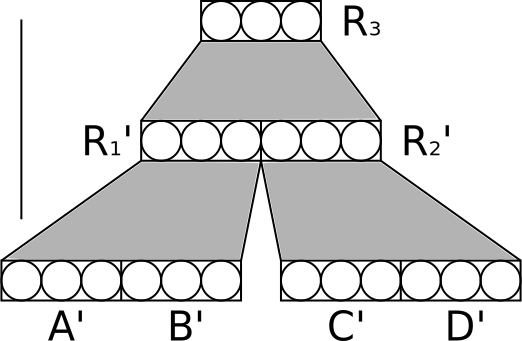
\includegraphics[scale=0.4]{img/raam_decode}
	\caption{Graph reconstruction from $x_3$ using trained RAAM model}
	\label{fig:raam_reconstruction}
\end{center}
\end{figure}



A significant feature of the RAAM model is that a small reconstruction error in the case of non-terminal nodes may render the reconstruction of terminal nodes impossible. Therefore in the process of training a RAAM classifier it is necessary to set the acceptable reconstruction error value much smaller for the non-terminal nodes than for the terminal ones. A major drawback of the RAAM model is the \emph{moving target} problem. That is, a part of the learning set (the representations $x_1$ and $x_2$ from the example) changes during training. In such a case the training phase may not converge to an acceptable state~\cite{goulon2005hopfield}. However, a different training schema is possible, based on recurrent neural networks training procedure~\cite{goulon2005hopfield}. A processing graph is built out of instances of the compressor and reconstructor units (Fig.~\ref{fig:raam_tree}), with structure reflecting the structure of the processed graph (if the dataset consists of multiple graphs, such procedure is repeated for every graph in the dataset). All instances of the compressor unit share their weights and all instances of the reconstructor unit share their weights - which is called the \emph{shared weights} technique. The labels of terminal nodes are fed to the processing network and the resulting error can be backpropagated using the Backpropagation Through Structure~\cite{kuchler1996inductive} algorithm (BPTS). It is worth noting, that the authors of such a modified RAAM model propose using an additional layer of hidden neurons in the compressor and reconstructor units. Such modification allows to partially separate the problem of the data model complexity (i.e. how complex should the RAAM model be to properly compress the data) from the size of terminal node labels which affect the number of input lines to the compressor unit.

\begin{figure}
\begin{center}
	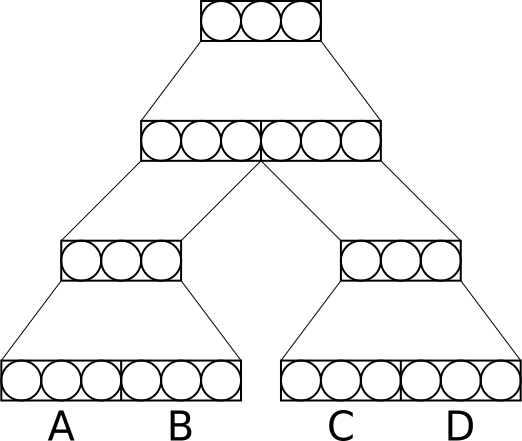
\includegraphics[scale=0.4]{img/raam_tree}
	\caption{Training RAAM using the BPTS procedure}
	\label{fig:raam_tree}
\end{center}
\end{figure}

The most important parameter of the RAAM model is the size of the encoded representation. On one hand, the size should be large enough to contain all the necessary compressed information about the encoded graph. On the other hand, it should be small enough for the compression mechanism to build a minimal representation, which stores only the necessary information about the dataset. If the size is too large, the trained model would store redundant information, memorizing the training set. This would result in a poor ability to process unseen data, which bear resemblance to the training set but is not the same. Experiments with natural language syntax processing~\cite{pollack1990recursive} proved that when the size of the compressed representation is accurate to the problem, the RAAM model is showing some constrained generalisation properties. A drawback of the standard RAAM approach is the termination problem. The model can't distinguish between terminal representations (node labels) and compressed representation which should be further reconstructed. To solve this problem, an additional encoding neuron can be introduced (increasing the representation size by one), which would take a different value for terminal and non-terminal representations~\cite{stolcke1992tree}.

\section{LRAAM}
The most important constraint of the RAAM model is the fact that only terminal nodes of the processed graphs (DPAGs) can contain labels. This problem was addressed by the Labeling RAAM model~\cite{sperduti1994labelling} (LRAAM, 1994), which separated the concepts of node labels and node representations. In the RAAM model the terminal nodes are represented by their labels. The LRAAM model introduced the concept of \emph{pointers}, which was used to describe a node representation which has to be learnt, regardless of whether the node is terminal or not. The pointers are built by compressor units (FNN with two or more layers) and they are decoded into graph structure by reconstructor units. More precisely, the pointer to $i$th node of the graph is calculated according to Eq.~\ref{eq:lraam_pointer}, where $x_i$ stands for pointer to the $i$th node, $f$ is the function implemented by the compressor unit, $l_i$ is the $i$th node label, $x_{ch_j}$ is the $j$th child node of $i$ and $k$ is the maximum outdegree of a node in the considered graph.

\begin{equation}
x_i = f(l_i, x_{ch_1}, .., x_{ch_k})
\label{eq:lraam_pointer}
\end{equation}

Whenever a node outdegree is smaller than $k$ (especially in the case of terminal nodes), the missing child pointers are substituted by the $NIL$ pointer, a special value representing the lack of node. The value of the node label is stacked together with all the pointers values to form an input vector which is fed to the compressor unit. The number of output neurons of the compressor unit (the size of a pointer $x_i$) is $m$. Let's denote the size of the label $l_i$ by $p$. The compressor unit must have $n = p + k \cdot m$ input lines which is also the number of reconstructor unit output neurons. The possibility of describing each graph node with its label provides a simple solution to the termination problem~\cite{sperduti1994labelling}. An additional value can be appended to each label, stating if the node is a terminal node or not. By using this method no interference with the LRAAM model is needed.

Just like the RAAM model, the LRAAM model experience the problem of the \emph{moving target}. The same technique of \emph{shared weights} can be applied, which results in building a large recursive neural network composed of identical units. A sample graph and the recursive network obtained by cloning the compressor and reconstructor units to match the sample graph structure are presented in Fig.~\ref{fig:lraam_tree}. As $A$ and $B$ are terminal nodes, their labels are fed to the compressor unit altogether with $NIL$ pointers representing the missing nodes. Then the compressed representation $x_{A}$ is built for node $A$ and the compressed representation $x_{B}$ is built for node $B$. The representations $x_A$ and $x_B$ are fed altogether with label $C$ to the compressor once again to build the representation $x_C$ of node $C$, which is also the representation of the whole graph.

\begin{figure}
\begin{center}
	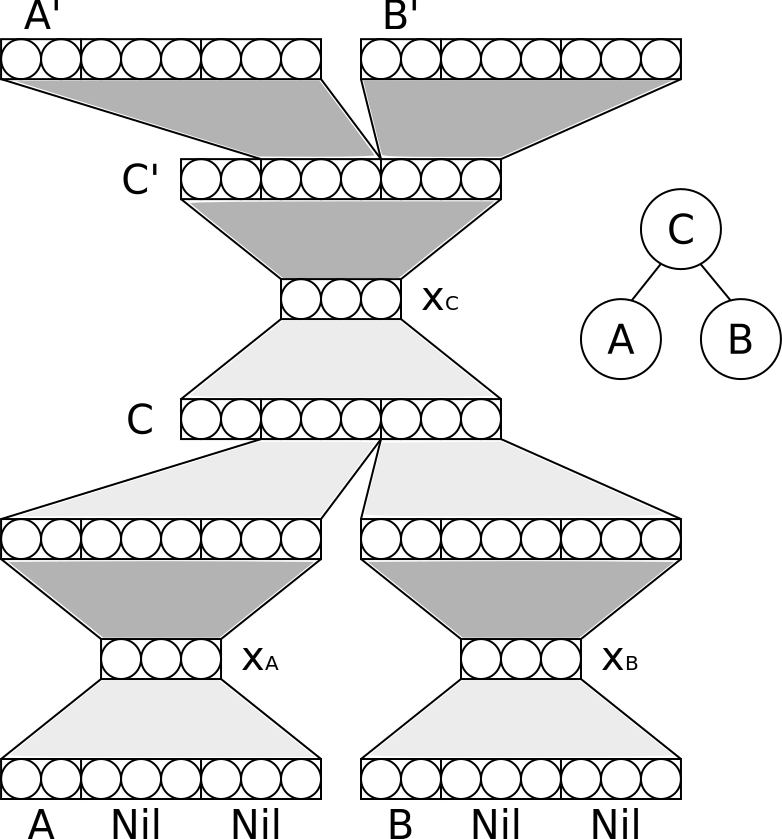
\includegraphics[scale=0.4]{img/lraam_tree}
	\caption{LRAAM encoding tree for the graph shown}
	\label{fig:lraam_tree}
\end{center}
\end{figure}

An extension of the LRAAM model exists for cyclic graphs. Whenever an edge forming a cycle is found, it is converted to a time unit delay. A sample cyclic graph and the resulting LRAAM model with one time delay was presented in Fig.~\ref{fig:lraam_tree_cycle}. The graph presented is similar to the graph used in the previous example, with the exception of the directed edge $A \Rightarrow C$. The additional edge forms a cycle so it must be represented as a time delay. Such an approach makes it possible to deal with cyclic graphs, however it is achieved at the expense of model simplicity. While with the shared weights technique it was possible to treat the encoding tree structure as a single feed-forward neural network with shared weights, with the time delays added the training of the network should consist of multiple time steps, up to a convergent state.

\begin{figure}
\begin{center}
	\includegraphics[scale=0.4]{img/lraam_tree_cycle}
	\caption{LRAAM encoding tree for the cyclic graph shown}
	\label{fig:lraam_tree_cycle}
\end{center}
\end{figure}

A distinctive feature of the LRAAM model is that a compressed representation is built for a given dataset (DPAGs) and the correctness of the representation is verified by mirroring the compression process and reconstructing the original data. When the obtained representation is accurate enough, the output of the LRAAM model is fed to a separate classifier which processes it and yields classification or regression results. The same applies to any new, unseen data, which is transformed by the trained LRAAM model and, if the model was built correctly, is compressed into a meaningful representation. Such separation of representation building and processing can be attractive for two reasons. First, the LRAAM model parameters, such as the size of the representation, can be tuned in a straightforward manner by observing what is the minimal value below which the original data cannot be accurately reconstructed from the compressed vectors. Secondly, any common classifier used for unstructured data can be used to process such compressed representation. On the other hand, it is often safe to presume that not all the data contained in node is crucial for the classification/regression process for which the compressed representation is needed. Such an approach lies beyond the standard LRAAM model and was introduced in the \emph{folding architecture} description~\cite{kuchler1996inductive}.


\section{Folding architecture and BPTS}
The ideas of \emph{folding architecture} and Backpropagation Through Structure (BPTS) were first introduced in 1996~\cite{goller1996learning}~\cite{kuchler1996inductive}. The model of the folding architecture is similar to that of LRAAM and is capable of processing rooted DPAGs. The folding architecture model is a feed-forward, fully connected multi-layer neural network, consisting of two subsequent parts performing different tasks: the \emph{folding} network and the \emph{transformation} network. The folding network is similar to the LRAAM compressor unit, its input layer consists of $p + k \cdot m$ input lines, $p$ for the processed node label and $k \cdot m$ for the compressed representations of the nodes children. The folding network can consist of any number of sigmoid neuron layers and its last layer produces the node compressed representation of size $m$. The folding network is applied to every node in the graph, starting from the leaves to provide the internal graph nodes with compressed representations of previous layers nodes. The transformation network is applied to the root node only. It can consist of any number of sigmoid neuron layers and an output layer. It takes as input the compressed representation of the root node and produces for it an output, which should match the expected output for a graph. Therefore, the transformation network is used to perform classification or regression tasks in terms of whole graphs.

The original idea behind the \emph{folding architecture} is that the compressed representation is built only for classification purpose and is fed directly to the transformation network. The output of the transformation network is then compared with the expected output and the error can be backpropagated through the folding architecture network by using a gradient-descent procedure, Backpropagation Through Structure. BPTS was invented as a generalisation of the Backpropagation Through Time method (BPTT~\cite{pineda1987generalization}), which in turn was invented for error backpropagation in recurrent neural networks. It can be described in terms of the \emph{unfolded} network. The unfolded network is never built physically but can be imagined as a graph built of folding network instances and reflecting the structure of the processed graph, with the transformation network added on top of it (attached to the representation of the root node). An unfolding network for a sample graph is presented in Fig.~\ref{fig:virtual_unfolding}. The light grey areas are instances of the folding network, while the dark grey area is the transformation network, which for the root node $C$ produces output $o_C$.

\begin{figure}
\begin{center}
	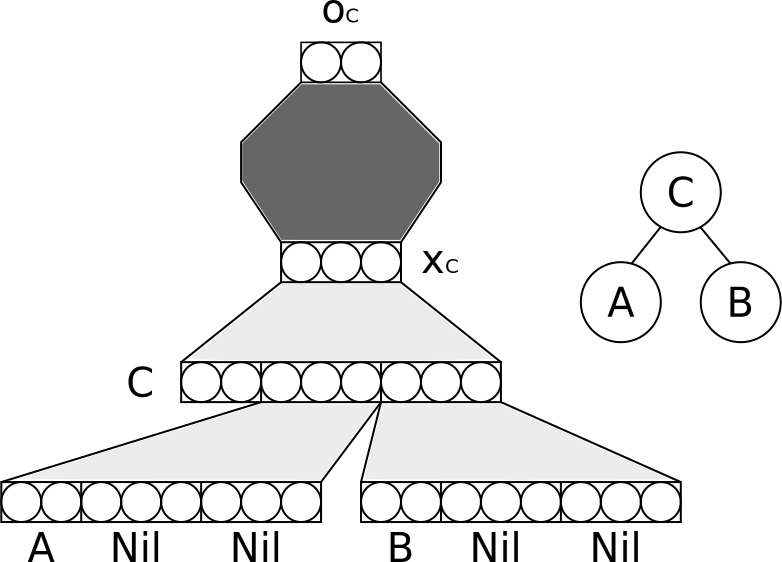
\includegraphics[scale=0.4]{img/virtual_unfolding}
	\caption{Virtual unfolding, reflecting the sample graph structure}
	\label{fig:virtual_unfolding}
\end{center}
\end{figure}

To explain the idea of BPTS it is necessary to briefly summarize the idea of BPTT (a detailed explanation can be found in RNN-concerned publications, e.g.~\cite{williams1995gradient}). Let's consider a fully-connected recurrent neural network, designed for classifying sequences of samples of size $m$. The network consists of a single layer of $n$ units with $n \times n$ recurrent connections, producing an output $y(t)$ at time $t$. Let $x^{s}(t)$ denote the $m$-tuple of input signals corresponding to the sample fed at time $t$. Further, let $x(t)$ be the merged input fed to the next network at time $t$, obtained by concatenating the vectors $x^{s}(t)$ and $y(t)$. To distinguish between the elements of vector $x_t$ corresponding to $x^{s}(t)$ and to $y(t)$, let's introduce two subsets of indices: $I$ and $U$ (Eq.~\ref{eq:bptt_indices}).

\begin{equation}
x_k(t) = \left\{
\begin{array}{l l}
	x^{s}_{k}(t)	& \quad \text{if $k \in I$} \\
	y_k(t)	& \quad \text{if $k \in U$}\\
\end{array} \right.
\label{eq:bptt_indices}
\end{equation}

\noindent Let $w_{ij}$ denote the network weight on connection to the $i$th neuron from input $x_j$, $net_k(t)$ denote the weighted sum of neuron inputs fed to the activation function $f_k$ (Eq.~\ref{eq:bptt_netk}).
\begin{equation}
net_k = \sum_{l \in (I \cup U)} w_{lk} x_l
\label{eq:bptt_netk}
\end{equation}

\begin{equation}
y_k = f_k(net_k)
\label{eq:bptt_f}
\end{equation}

\noindent Let's consider a recurrent network which was operating from a starting time $t_0$ up to time $t$. We may represent the computation process performed by the network by \emph{unrolling} the network in time, that is building a feed-forward neural network made of identical instances of the considered recurrent neural network, one instance per time step $\tau$, $\tau \in (t_0, t]$.. To compute the gradient of $J(t)$ at time $t$ it is necessary to compute values $\epsilon_k(\tau)$ and $\delta_k(\tau)$ for $k \in U$ and $\tau \in (t_0, t]$ by means of equations~\ref{eq:bptt_epsilon},~\ref{eq:bptt_delta} and~\ref{eq:bptt_summaric}.

\begin{equation}
\epsilon_k(t) = e_k(t)
\label{eq:bptt_epsilon}
\end{equation}

\begin{equation}
\delta_k(\tau) = f'_k(net_k(\tau))\epsilon_k(\tau)
\label{eq:bptt_delta}
\end{equation}

\begin{equation}
\epsilon_k(\tau - 1) = \sum_{l \in U} w_{lk} \delta_l(\tau)
\label{eq:bptt_summaric}
\end{equation}

\noindent At time $t$ an external error $e(t)$ is \emph{injected} to the network, presumably being the difference between the trained network output at time $t$ and the expected output. The following steps compute the error $\epsilon(\tau)$ by backpropagating the original error through the layers of the unrolled neural network.

The BPTS method implements the BPTT algorithm. Backpropagation starts at the last layer of the virtual unfolding network, where the classification/regression error is calculated. The error is injected to the last layer of the transformation network of the root node and backpropagated using the BPTT algorithm down to the first layer of the folding network of the root node. The error is then backpropagated from there to the last layers of virtually connected root child nodes, as if there were physical connections between the two layers. Such backpropagation continues down to the first layers of folding network applied to terminal nodes (leaves).

The folding architecture model introduced new important ideas in the domain of connectionist graph processing models. First of all, the representation building model is simpler than the LRAAM model and the overall folding architecture was said to converge much faster than LRAAM for the same datasets~\cite{goller1996learning}. Secondly, three important concepts were adapted from the domain of recurrent neural networks: the error injection, BPTS and the unfolding of the network as a generalisation of unrolling a recursive neural network.


\chapter{Graph neural networks}
The Graph Neural Network model~\cite{scarselli2009graph} (GNN) is a quite recent (2009) connectionist model, based on recursive neural networks and capable of classifying almost all types of graphs. The main difference between the GNN model and previous connectionist models is the possibility of processing directly nonpositional and cyclic graphs, containing both node labels and edge labels. Although some similar solutions were introduced in an earlier model, the \emph{RNN-LE}~\cite{bianchini2005recursive} in 2005, it was the GNN model that combined several techniques with a novel learning schema to provide a direct and flexible method for graph processing.


\chapter{Experiments~\label{ch:experiments}}
Experiments were conducted to check if the implemented GNN is able to cope with the tasks presented in the original article~\cite{scarselli2009graph}. For all the experiments the state size was set to 5, the number of hidden neurons in both the $h_{\bm{w}}$ and $g_{\bm{w}}$ networks was set to 5. After a couple successful trivial experiments, consisting of memorizing a single graph, the proper experiments were conducted. The task chosen for experiments was the \emph{subgraph matching} task. It was chosen, because:
\begin{enumerate}
	\item a similar experiment was conducted by Scarselli et al.~\cite{scarselli2009graph}
	\item the dataset is easy to generate, yet the problem is not trivial
	\item to yield good results, the structure of the graph have to be exploited.
\end{enumerate}

\section{Subgraph matching - data}
The datasets for the subgraph matching task were generated as follows. For a given number of graph nodes, graphs were generated by selecting node labels from $[0..10]$ and then connecting each node pair in a graph with an edge probability $\delta$. Then, random edges were added to the graph until the graph became connected. Then, a smaller connected subgraph was inserted to every graph in the dataset. Then, a simple algorithm was used to locate all the copies of subgraph in every graph in the dataset. Thus, every graph in the dataset contained at least on copy of the subgraph. Afterwards, a small Gaussian noise with zero mean and standard deviation of $0.25$ was added to node labels. All the graph edges were undirected and thus were transformed to pairs of directed edges prior to processing. No edge labels were used.

Two datasets were generated. One with graph size (number of nodes) equal to 6, the subgraph size equal to 3 and $\delta = 0.8$ (100 graphs, called later the \emph{6-3 dataset}). The second one with graph size equal to 14, subgraph size equal to 7 and $\delta = 0.2$ (100 graphs, called later the \emph{14-7 dataset}). A larger $\delta$ was used for the first dataset, as graphs generated with $\delta = 0.2$ were mostly sequences. The first dataset was used to analyze the process of training, while the second one was used for comparison of GNN with a standard FNN classifier.

\section{Impact of initial weight values on learning}
To test the impact of initial weight values on the process of a GNN training, 9 different sets of weights were tested. For all tested networks, the contraction constant ($\mu$ from Eq.~\ref{eq:gnn_pw}) was set to $0.9$. The training was performed on 10 graphs belonging to the 6-3 dataset. Each GNN network was trained for 50 iterations. As the default error measure used for GNN training is the Mean Square Error, a connected performance measure - RMSE was used for evaluation. Results are presented in Fig.~\ref{fig:gnn_multiple}. Out of 9 networks, only 4 performed well: gnn2, gnn3, gnn5 and gnn7. The gnn5 network yielded the smallest RMSE at the end of training and also presents a remarkably monotonous RMSE slope compared with gnn7. All the other networks didn't improve significantly on the RMSE value, which may suggest that multiple initial values of weights should be tried for a given problem to build an efficient classifier.

\begin{figure}[h!]
\begin{center}
	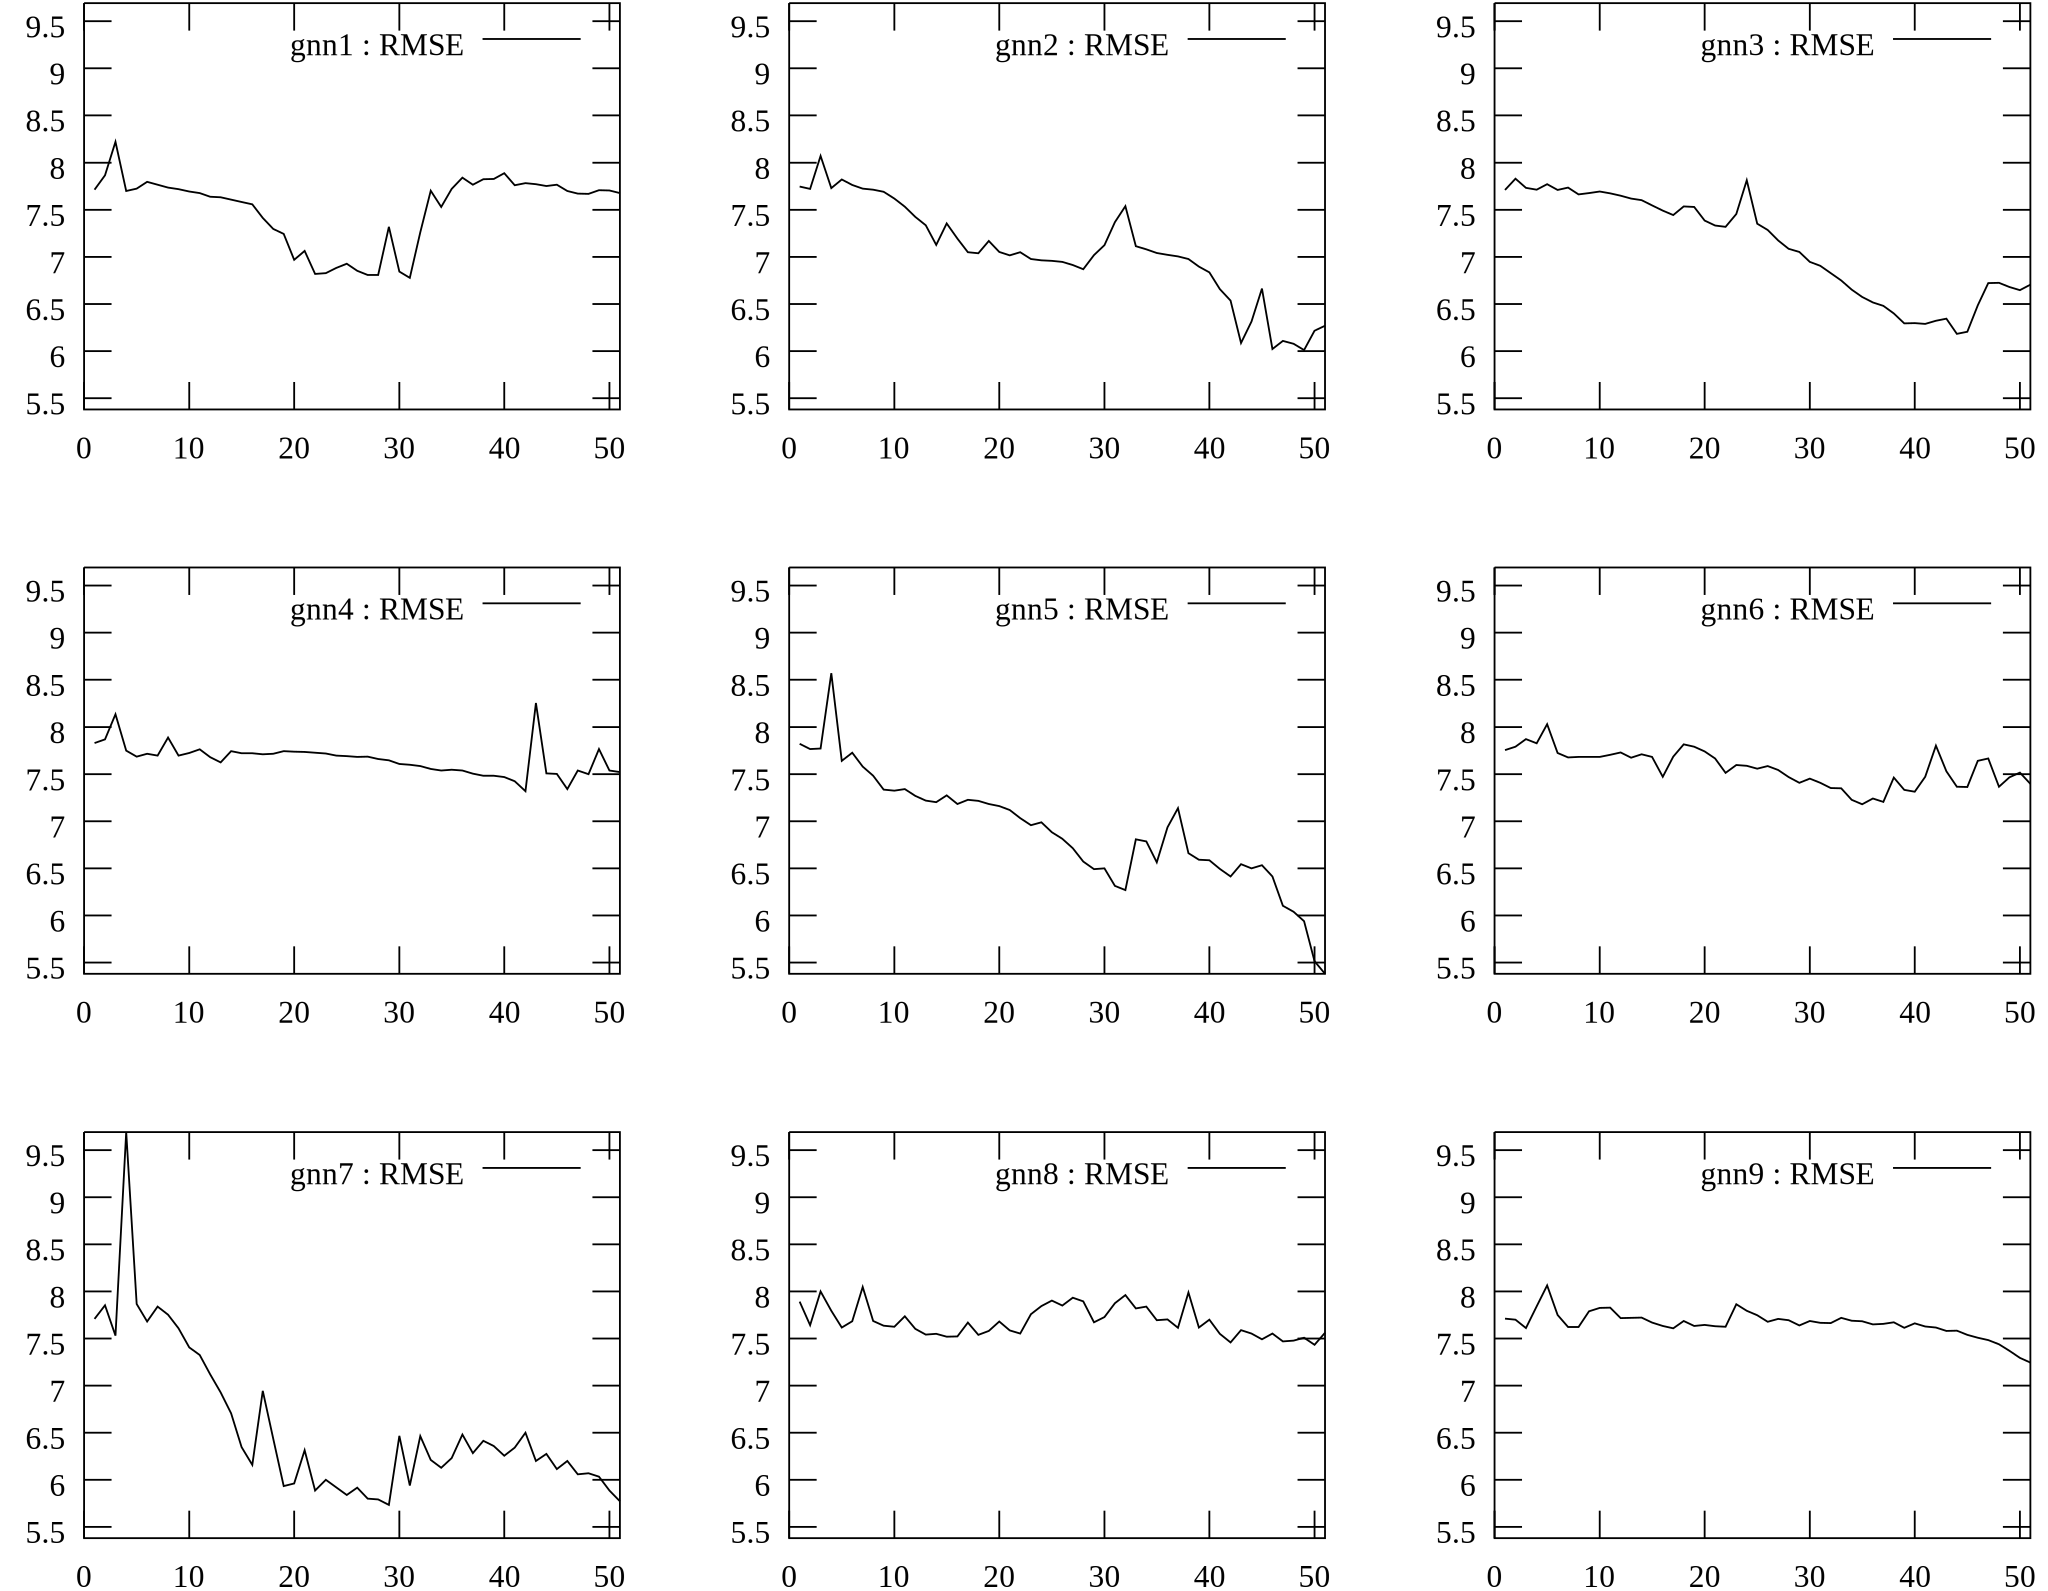
\includegraphics[scale=0.09]{img/rmse_gnn1-9}
	\caption{RMSE for 9 different initial weight sets. $\mu = 0.9$}
	\label{fig:gnn_multiple}
\end{center}
\end{figure}

\newpage
\section{Impact of contraction constant on learning}
During the initial experiments, interesting results were obtained for different values of the contraction constant ($\mu$ from Eq.~\ref{eq:gnn_pw}). It seems that for a given learning task exists a minimum value of $\mu$ below which no learning occurs. Some experiments were conducted for the 6-3 dataset using the best networks from Fig.~\ref{fig:gnn_multiple}: the gnn5 and gnn7 network (initial weights were used). The results for gnn5 are presented in Fig.~\ref{fig:gnn5} and the results for gnn7 are presented in Fig.~\ref{fig:gnn7}. For both networks three different value of $\mu$ were tested: 1.2, 0.9 and 0.6. In both cases it can be observed that no training occurs for $\mu = 0.6$. For these experiments 20 graphs from the 6-3 dataset were used.

\begin{figure}[h!]
\begin{center}
	\includegraphics[scale=0.09]{img/rmse_clipped}
	\caption{RMSE for gnn5 with $\mu \in [1.2, 0.9, 0.6]$}
	\label{fig:gnn5}
\end{center}
\end{figure}

\begin{figure}[h!]
\begin{center}
	\includegraphics[scale=0.09]{img/rmse1_clipped}
	\caption{RMSE for gnn7 with $\mu \in [1.2, 0.9, 0.6]$}
	\label{fig:gnn7}
\end{center}
\end{figure}

A closer look on the process of learning may shed some light on the reasons behind the lack of learning. In Fig.~\ref{fig:gnn7_09} the process of learning of gnn7 with $\mu = 0.9$ are presented. In Fig.~\ref{fig:gnn7_06} the same network gnn7 was trained with $\mu = 0.6$. The different values shown are: \emph{nForward} - number of \emph{Forward} state building iterations, \emph{nBackward} - number of \emph{Backward} error accumulation iterations, \emph{penalty} - was any weight penalized, \emph{de/dw influence} - percent of combined weight updates that had the sign same as $\frac{\partial e}{\partial w}$ (before passing to RPROP algorithm), \emph{dp/dw influence} - percent of combined weight updates that had the sign same as $\frac{\partial p}{\partial w}$. Some interesting features of the GNN model learning schema can be observed. In the case of $\mu = 0.9$ the number of \emph{Forward} steps reached the maximum a couple of times, which presumably means that at that time the $F_{\bm{w}}$ ceased being a contraction map. The penalty was imposed mostly for short periods of time and only at one moment caused the $\frac{\partial e}{\partial w}$ influence to drop below 50\%. This strategy yielded good results - the penalty imposed reduced the number of \emph{Forward} steps and the RMSE was successfully reduced.

\begin{figure}[h!]
\begin{center}
	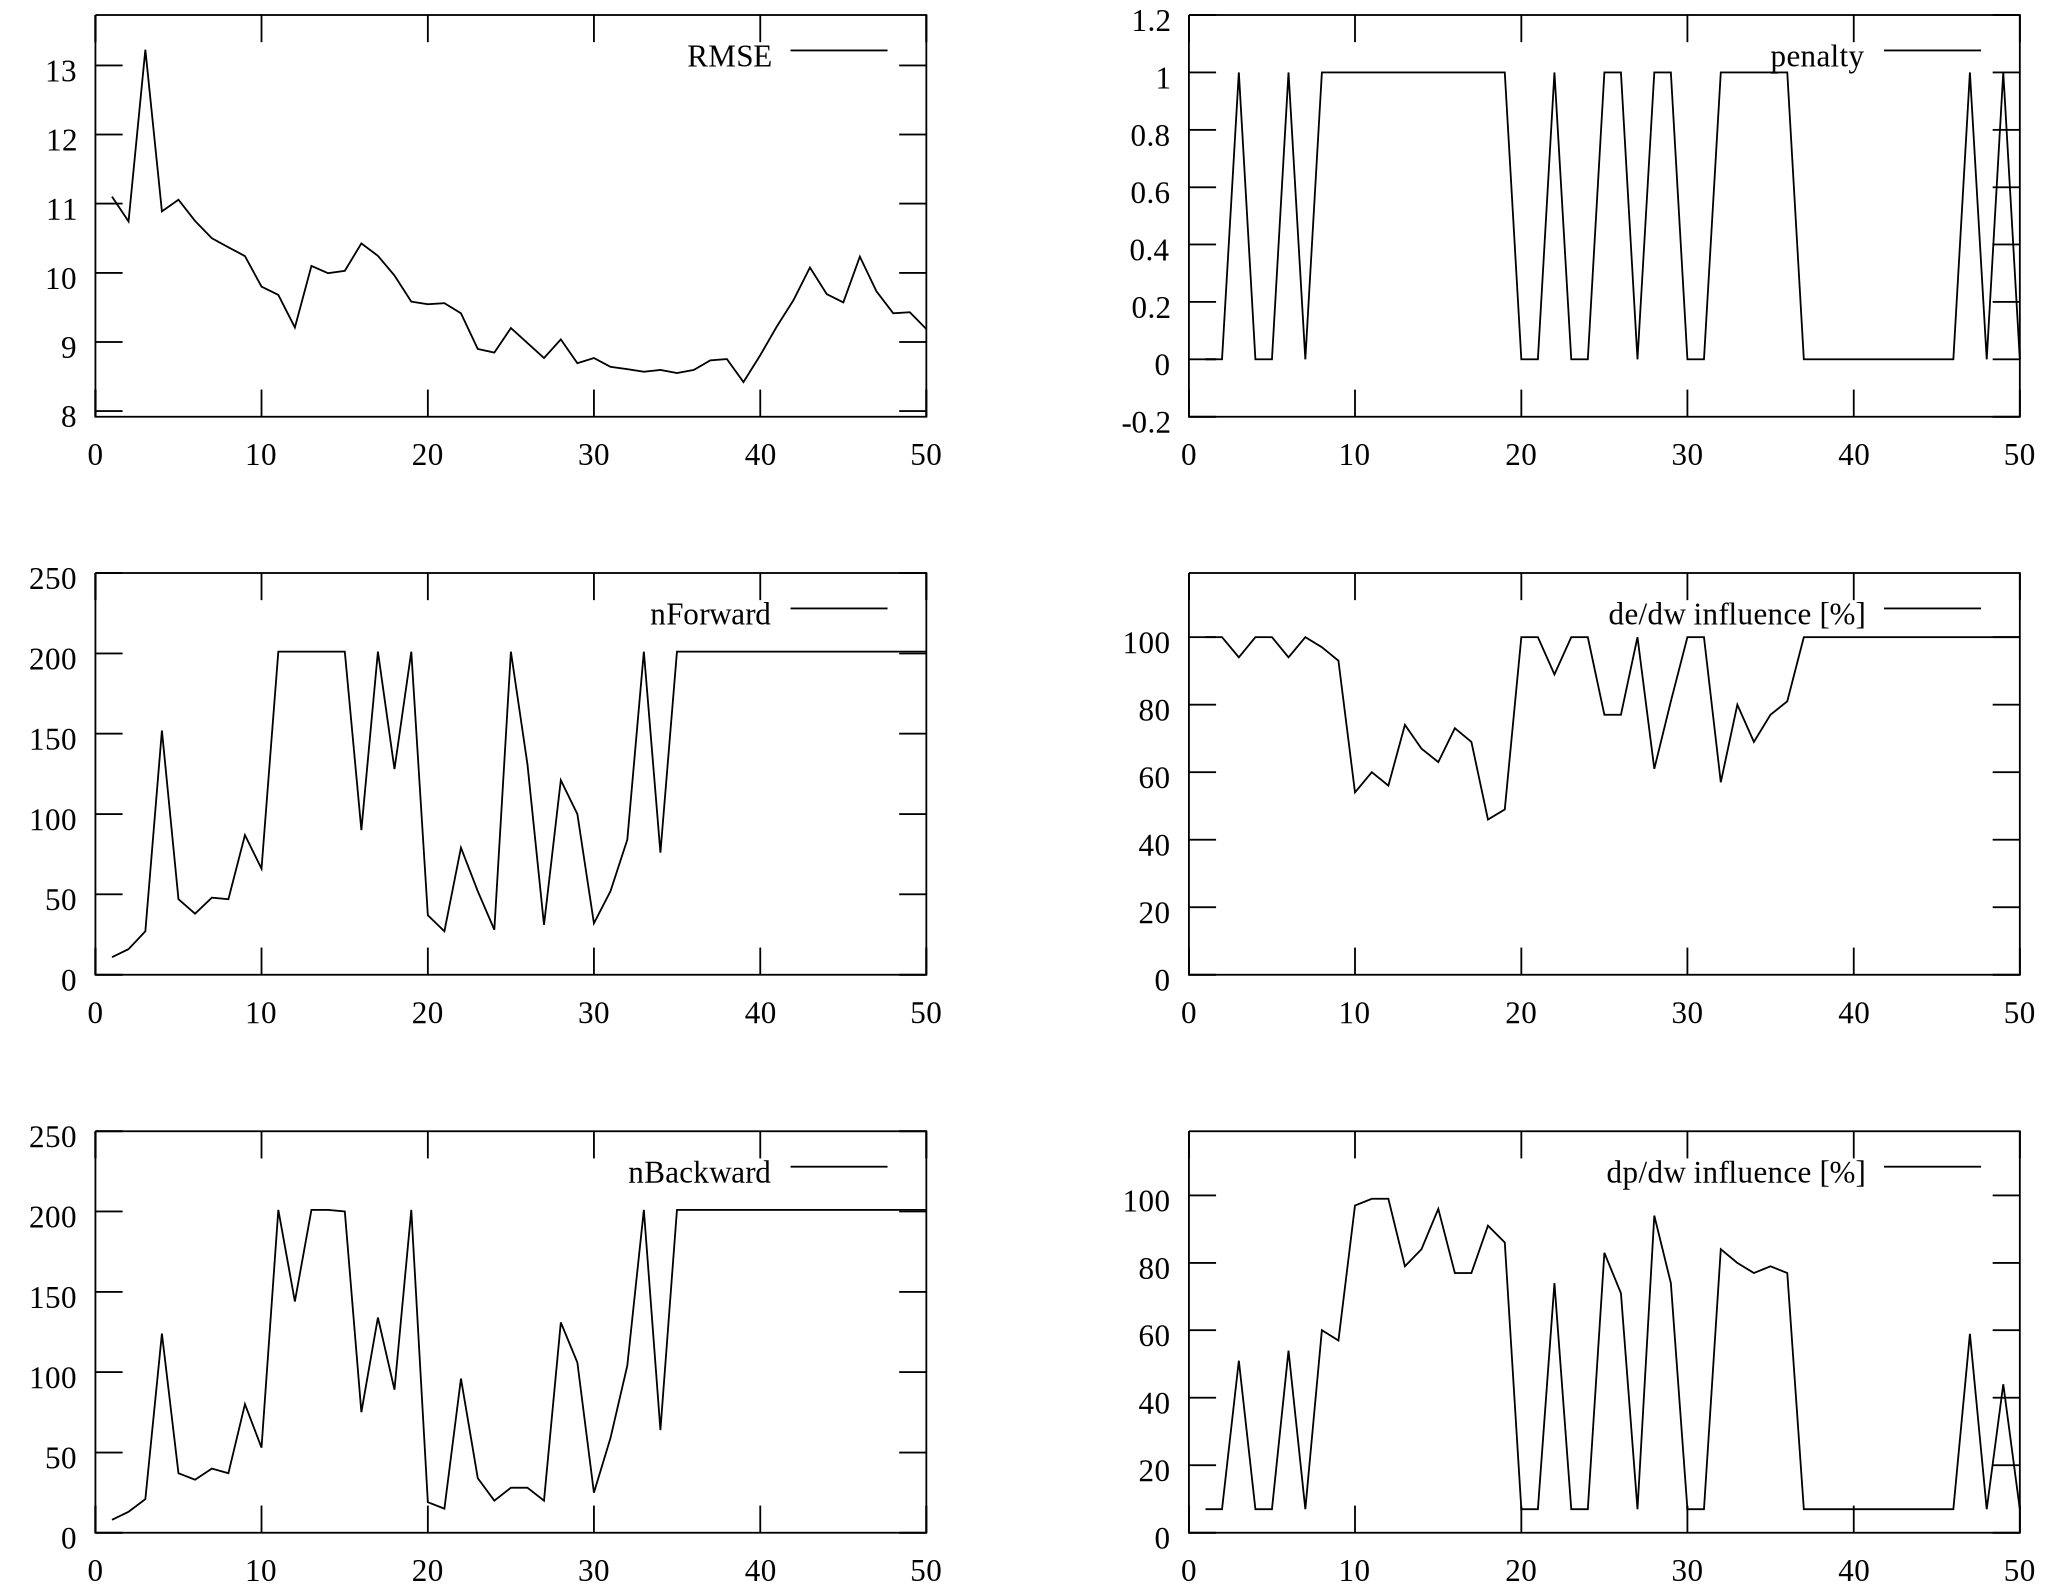
\includegraphics[scale=0.09]{img/gnn1_2}
	\caption{gnn7 performance with $\mu = 0.9$}
	\label{fig:gnn7_09}
\end{center}
\end{figure}

A different situation is shown for $\mu = 0.6$. Because of a low $\mu$ value, the penalty was imposed hastily and was larger than in the previous case (the impact of the $\mu$ value was shown in Eq.~\ref{eq:gnn_pw_L}). It was imposed even when the number of \emph{Forward} steps was below the maximum, that is when $F_{\bm{w}}$ was still a contraction map. Large values of the penalty caused a huge decrease of the $\frac{\partial e}{\partial w}$ term influence, which made any learning impossible.

\begin{figure}[h!]
\begin{center}
	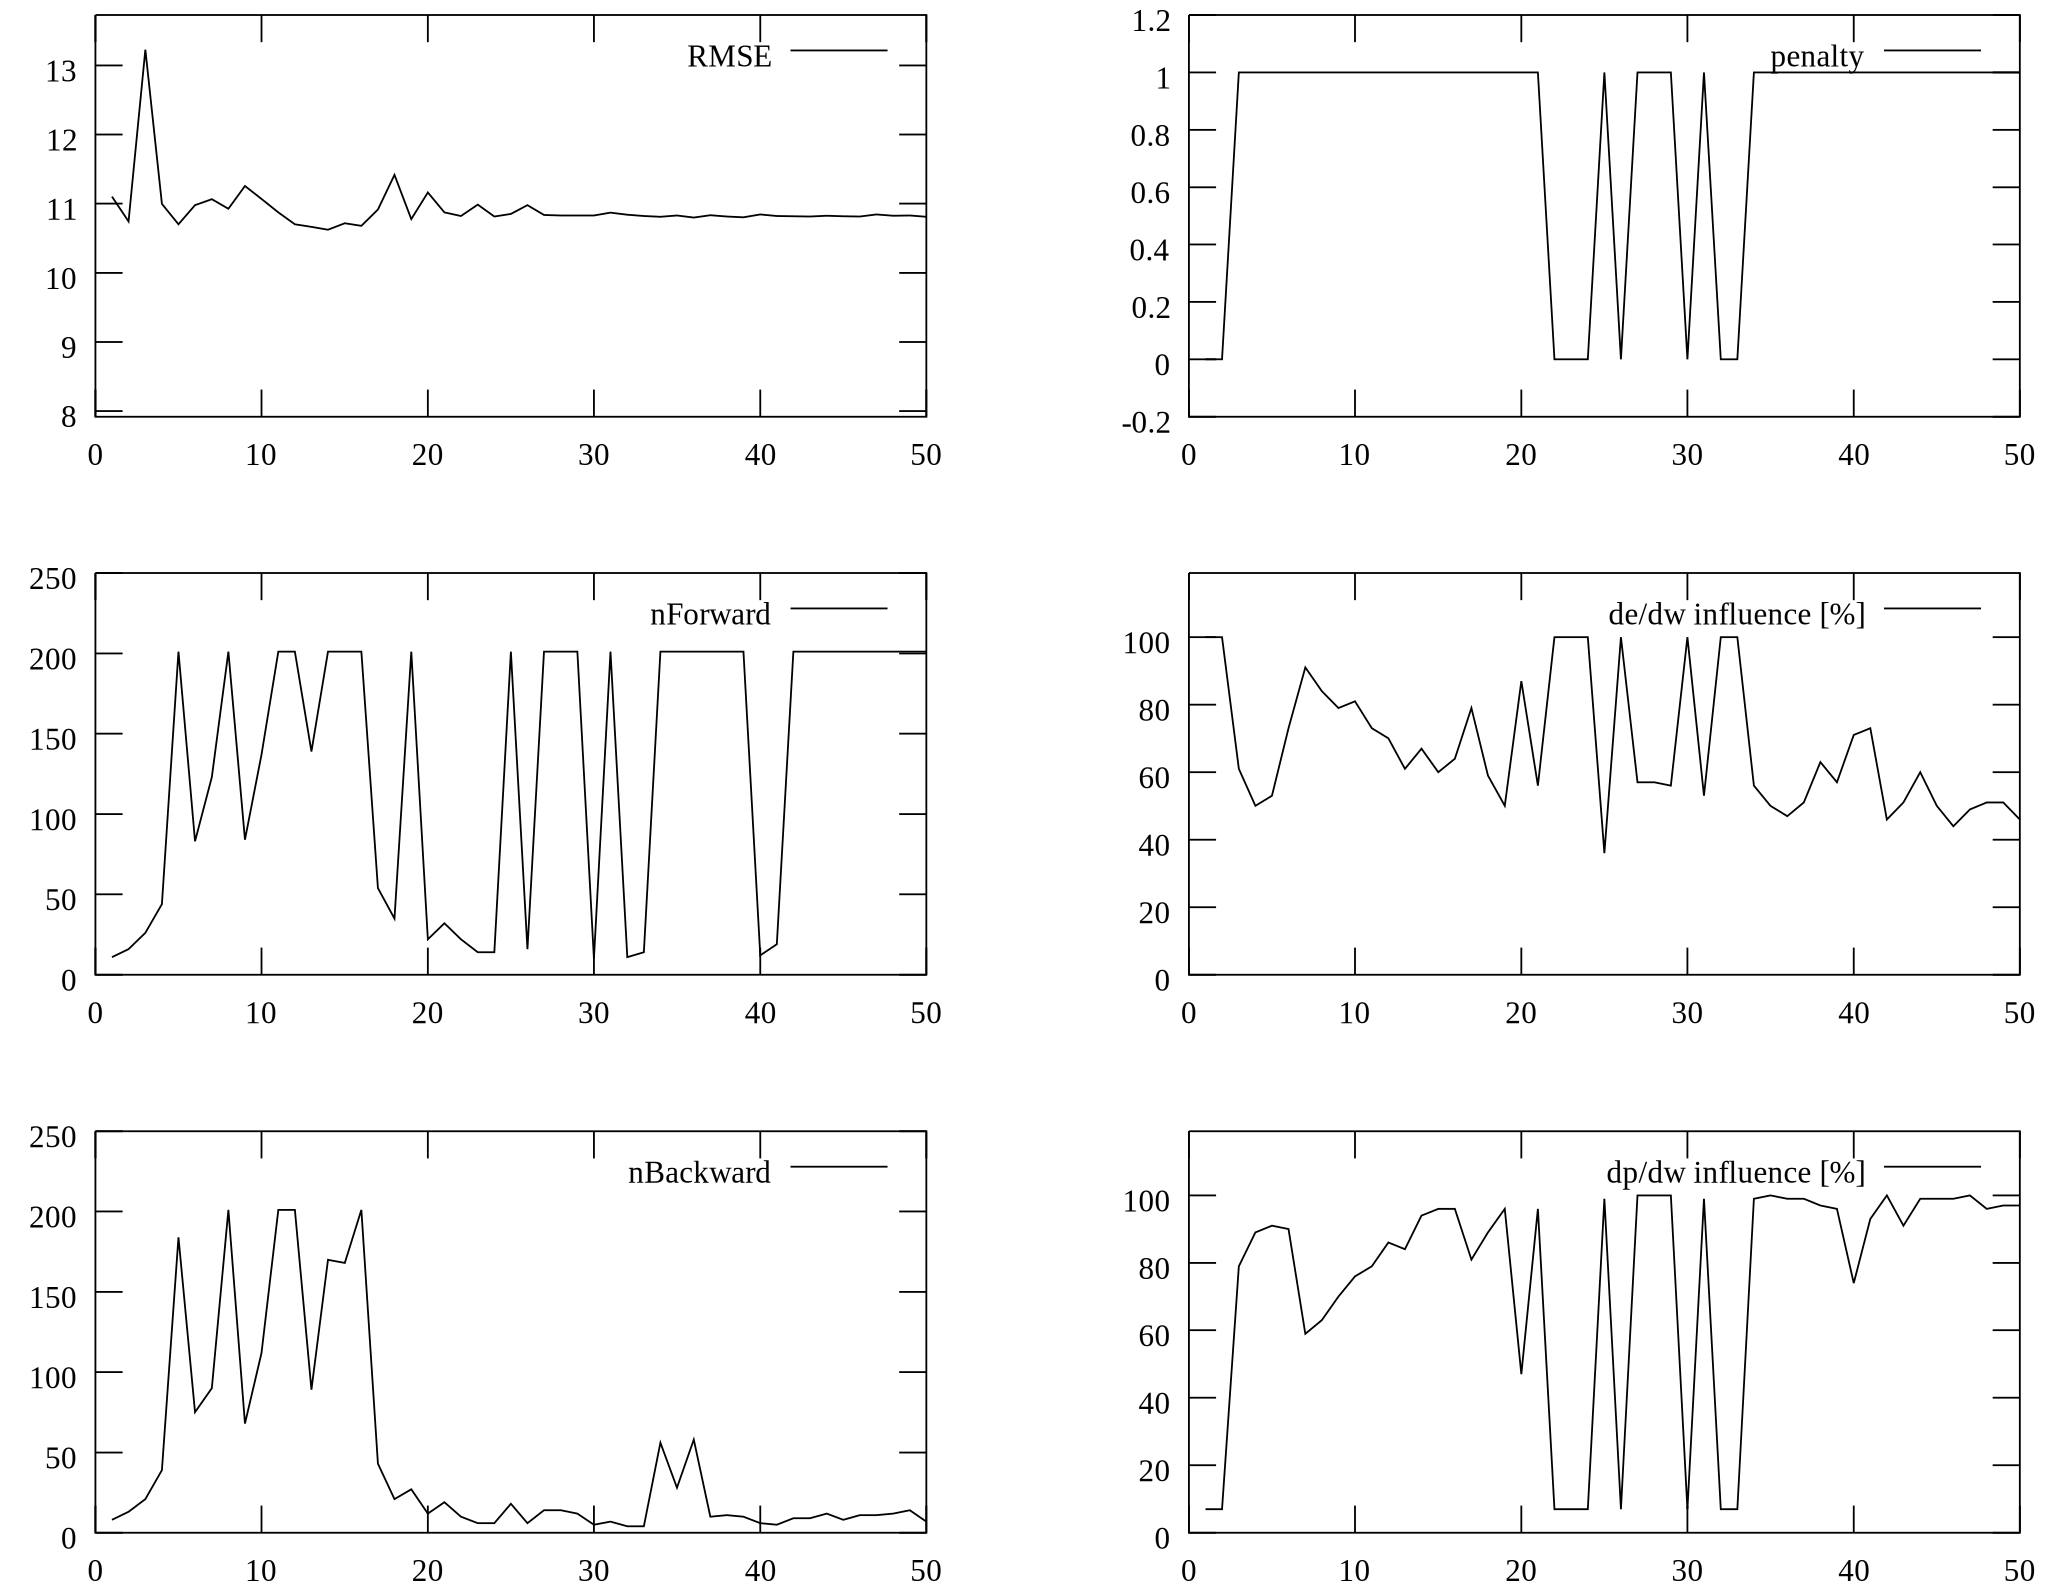
\includegraphics[scale=0.09]{img/gnn1_3}
	\caption{gnn7 performance with $\mu = 0.6$}
	\label{fig:gnn7_06}
\end{center}
\end{figure}

\newpage
Another interesting case is presented in Fig.~\ref{fig:gnn5_09}. The learning process of gnn5 on 10 graphs with $\mu = 0.9$ is presented. It can be observed that even as the number of \emph{Forward} steps reached in peaks the maximum value, the $F_{\bm{w}}$ function remained a contraction map. A large enough $\mu$ prevented the penalty from being imposed, which enabled the GNN model to train both computation units without any disturbance. The result is a monotonously decreasing RMSE slope, which could be previously observed in Fig.~\ref{fig:gnn_multiple}. It can be concluded, that the most important aspect of building a GNN model is to provide an efficient way to make $F_{\bm{w}}$ a contraction map as fast as possible, so as to provide as much time as possible for undisturbed learning.

\newpage
\begin{figure}[h!]
\begin{center}
	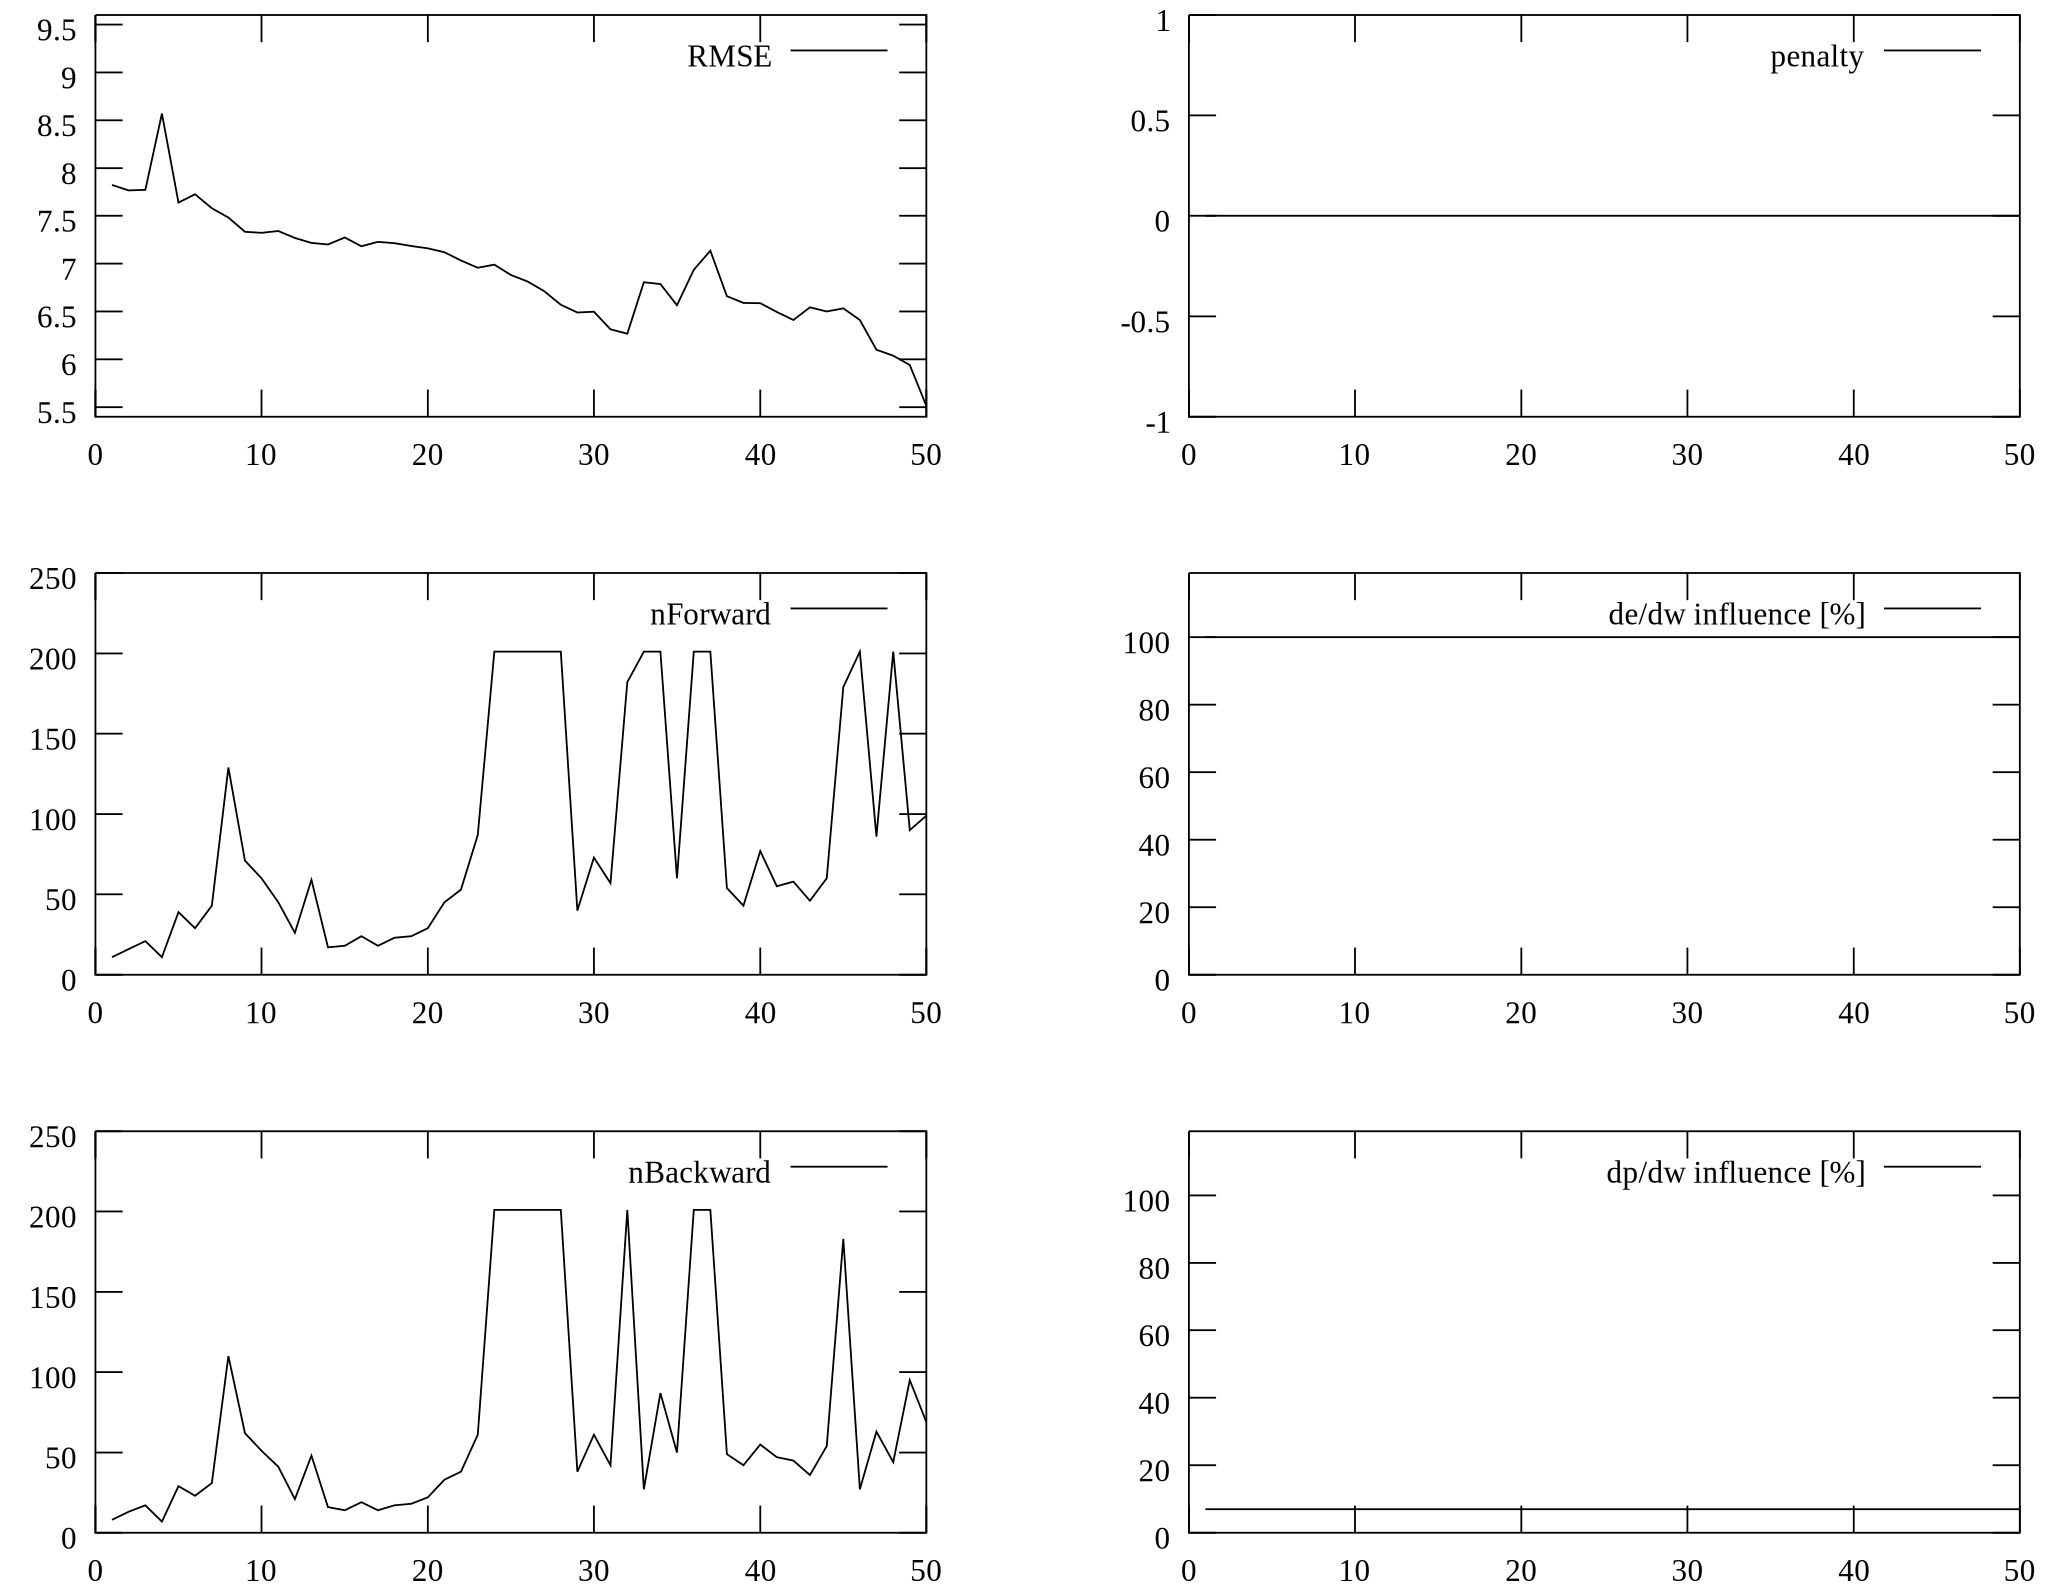
\includegraphics[scale=0.09]{img/gnn5}
	\caption{gnn5 performance with $\mu = 0.9$}
	\label{fig:gnn5_09}
\end{center}
\end{figure}

\newpage
\section{Crossvalidation results}
To present the performance of the implemented GNN model compared to the performance of a standard FNN, the following subgraph matching experiment was conducted. 5-fold crossvalidation was performed on all 100 graphs from the 14-7 dataset. A random GNN was used with contraction constant $\mu = 0.9$ and it was trained from scratch for 50 iterations during each fold. To provide good FNN results, 10 three-layer FNNs with 5 hidden $tanh$ neurons were evaluated and the one with best mean accuracy was selected. The results are presented in Table~\ref{tab:crossmean} and~\ref{tab:crossstd}. It can be seen that the GNN classifier outperformed the FNN by as much as 20\%. This is due to the fact, that the FNN classifier could make predictions only by analyzing node labels, while the GNN classifier exploited correctly the graph topology.

These results can be better understood by analyzing the classified dataset. The 100 processed graphs consisted in total of 1400 nodes. Amongst these nodes, 1031 had node labels matching the subgraph node labels. Amongst these 1031 nodes only 702 actually belonged to the subgraph. Thus, 329 nodes, 23.5\% of all the nodes would probably be classified as false positives by a classifier taking into consideration only node labels. This hypothesis corresponds quite well with the results presented.

\begin{table}[h!]
	\begin{center}
	\begin{tabular}{llll}
	\toprule
	& accuracy & precision & recall \\
	\midrule
	FNN - tr &	71\% &  65\% & 93\% \\
	FNN - tst &	71\% &  64\% &  93\% \\
	GNN - tr &	91\% &  87\%&  97\% \\
	GNN - tst &	91\% &  86\% &  97\% \\
	\bottomrule
	\end{tabular}
	\caption{Mean values on training and test sets}
	\label{tab:crossmean}
	\end{center}
\end{table}

\begin{table}[h!]
	\begin{center}
	\begin{tabular}{llll}
	\toprule
	& accuracy & precision & recall \\
	\midrule
	FNN - tr &	0.34\% &  0.67\% & 1.86\% \\
	FNN - tst &	2.45\% &  1.73\% &  2.93\% \\
	GNN - tr &	1.62\% &  1.71\% &  2.07\% \\
	GNN - tst &	3.06\% &  3.70\% &  1.39\% \\
	\bottomrule
	\end{tabular}
	\caption{Standard deviations on training and test sets}
	\label{tab:crossstd}
	\end{center}
\end{table}


\appendix

\listoftables
\listoffigures

% tutaj załączniki

%\nocite{*}
%\bibliographystyle{plplain}
\bibliographystyle{ieeetr}
%\bibliographystylebk{plplain}
%\bibliographystylest{plplain}
%\bibliographystyledoc{plplain}
% \bibliographystyleweb{plplain}
%\bibliographybk{BIB/books}
%\bibliographyst{BIB/books}
%\bibliographydoc{BIB/books}
% \bibliographyweb{BIB/books}

\bibliography{bib/gnn}

\end{document}

% ex: set tabstop=4 shiftwidth=4 softtabstop=4 noexpandtab fileformat=unix filetype=tex spelllang=pl,en spell:

